\section{Architetture}
\subsection{Architetture a livelli}
\begin{itemize}
	\item \textbf{Architettura ad un livello}: L'unico livello fisico è quello delle sorgenti. Questa architettura non è giudicata buona perché il lavoro (le operazioni OLAP) ricadrebbero appunto sui DB sorgenti, ovvero quelli operazionali, portando malcontento generale.
	\begin{figure}[H]
		\begin{center}
			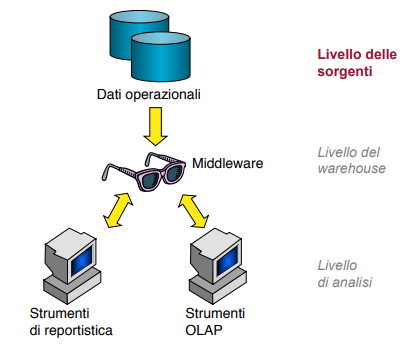
\includegraphics[width=0.4\linewidth]{img/onelevel.PNG}
			\caption{Architettura a un livello}
		\end{center}
	\end{figure}
	\item \textbf{Architettura a due livelli}: I due livelli fisici sono il livello delle sorgenti e quello del Data Warehouse. Si aggiunge quindi una nuova base di dati, che viene popolata a intervalli di tempo regolare attraverso l'ETL. I metadati sono dati che descrivono la forma dei dati all'interno del Data Warehouse. A partire da questa architettura le soluzioni a livelli sono giudicate tutte buone e vengono implementate in base alle esigenze dell'azienda che le richiede.
	\begin{itemize}
		\item A livello del warehouse è continuamente disponibile informazione di buona qualità anche quando, per motivi tecnici oppure organizzativi, è temporaneamente precluso l’accesso alle sorgenti;
		\item L’interrogazione analitica effettuata sul Data Warehouse non interferisce con la gestione delle transazioni a livello operazionale, la cui affidabilità è essenziale per il funzionamento dell’azienda;
		\item L’organizzazione logica del Data Warehouse è basata sul modello multidimensionale, mentre le sorgenti offrono in genere modelli relazionali o semi-strutturati;
		\item C’è una discordanza temporale e di granularità tra sistemi OLTP, che trattano dati correnti e al massimo livello di dettaglio, e sistemi OLAP che operano su dati storici e di sintesi;
		\item A livello del warehouse è possibile impiegare tecniche specifiche per ottimizzare le prestazioni per applicazioni di analisi e reportistica.
	\end{itemize}
	\begin{figure}[H]
		\begin{center}
			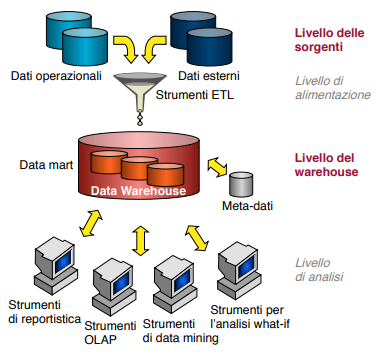
\includegraphics[width=0.4\linewidth]{img/twolevel.PNG}
			\caption{Architettura a due livelli}
		\end{center}
	\end{figure}
	\item \textbf{Architettura a tre livelli}: I tre livelli fisici sono quello delle sorgenti, quello del Data Warehouse e quello di alimentazione, ossia quello in cui c'è l'ODS.
	\begin{itemize}
		\item Il vantaggio principale del livello dei dati riconciliati è che esso crea un modello di dati comune e di riferimento per l’intera azienda, introducendo al contempo una separazione netta tra le problematiche legate all’estrazione e integrazione dei dati dalle sorgenti e quelle inerenti l’alimentazione del DW;
		\item Unico difetto è il maggior consumo di spazio, dovuto all’ulteriore ridondanza che si crea rispetto ai dati operazionali sorgente.
	\end{itemize}
	\begin{figure}[H]
		\begin{center}
			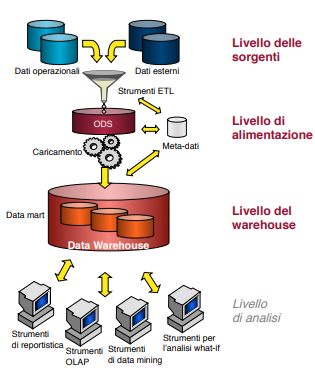
\includegraphics[width=0.4\linewidth]{img/threelevel.PNG}
			\caption{Architettura a tre livelli}
		\end{center}
	\end{figure}
\end{itemize}
\subsection{Architetture non a livelli}
\begin{itemize}
	\item \textbf{Data Mart indipendenti}: Esistono diversi Data Mart indipendenti che però spesso non riescono a "parlarsi". Si tratta dell'architettura più semplice da realizzare, ma il rischio è che i Data Mart, essendo sviluppati in momenti diversi potrebbero non essere consistenti tra loro e mostrare dati in maniera non consistente. Diventa quindi impossibile effettuare delle query cross, ovvero sfruttando tutti i Data Mart.\newline
	Questa soluzione è quindi giudicata NON buona in quanto non rispetta il requisito del Data Warehouse "\textit{Integrato e consistente}".
	\begin{figure}[H]
		\begin{center}
			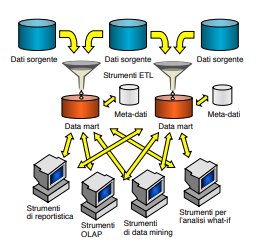
\includegraphics[width=0.4\linewidth]{img/indipendent.PNG}
			\caption{Architettura a Data Mart indipendenti}
		\end{center}
	\end{figure}
	\item \textbf{Data Mart Bus}: Simile alla soluzione \textit{"Data Mart indipendenti"}, ma i Data Mart sono collegati tra loro attraverso un bus logico. Questo è possibile accordandosi preventivamente su alcuni standard da mantenere durante la progettazione di un Data Mart. In questo modo i Data Mart possono essere creati in momenti diversi, ma sono vincolati e devono rispettare le specifiche preventivamente definite in modo da poter effettuare query cross. I caratteri e i livelli di dettaglio di un determinato concetto sono quindi sempre gli stessi. Possiamo vedere questa operazione come una specie di "join" tra Data Mart.
	\begin{figure}[H]
		\begin{center}
			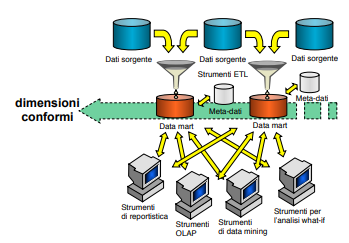
\includegraphics[width=0.5\linewidth]{img/bus.PNG}
			\caption{Architettura Data Mart Bus}
		\end{center}
	\end{figure}
	\item \textbf{Hub-and-spoke}: In questo caso esiste un ODS enterprise (il suo scope è l'intera azienda). Esistono quindi tanti Data Mart che sono per forza integrabili tra loro, in quanto i loro dati arrivano dallo stesso Database riconciliato. Si tratta di un'architettura molto più complessa e costosa da realizzare, a causa dell'ODS.
	\begin{figure}[H]
		\begin{center}
			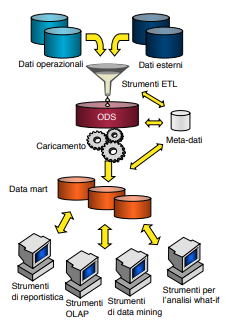
\includegraphics[width=0.35\linewidth]{img/hubspoke.PNG}
			\caption{Architettura Hub-and-spoke}
		\end{center}
	\end{figure}
	\item \textbf{Federazione}: Utilizzato nel caso in cui per esempio una grossa azienda acquista altre aziende le quali dispongono già di un Data Warehouse. Risulterebbe estremamente costoso ricreare un unico Data Warehouse "riconciliato" da zero, quindi si crea un Data Wareouse ulteriore, ad un altro livello. Ci sono altrettanti ETL che trasformano i dati e mandano tutto al Data Warehouse di secondo livello.\newline
	I Data Mart in questo caso sono sylos, non condividono tra loro informazioni, proprio perché sono stati progettati in modo differente.\newline
	In questo caso la complessità di sposta sulla creazione dell'ETL.\newline
	Questa architettura serve solo in contesti particolari.
	\begin{figure}[H]
		\begin{center}
			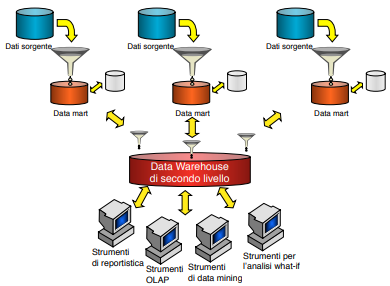
\includegraphics[width=0.5\linewidth]{img/federation.PNG}
			\caption{Architettura Federazione}
		\end{center}
	\end{figure}
\end{itemize}

\noindent Le quattro principali aziende che offrono queste soluzioni sono IBM, Oracle, SAP e Microsoft. L'architettura viene scelta in base al contesto e ai bisogni dell'azienda. Solitamente si adottano soluzioni enterprise e non open source in quanto non c'è competizione in quanto servizio offerto.
